%!TEX root = thesis.tex

%\begin{figure}[ht]
%	\centering
%  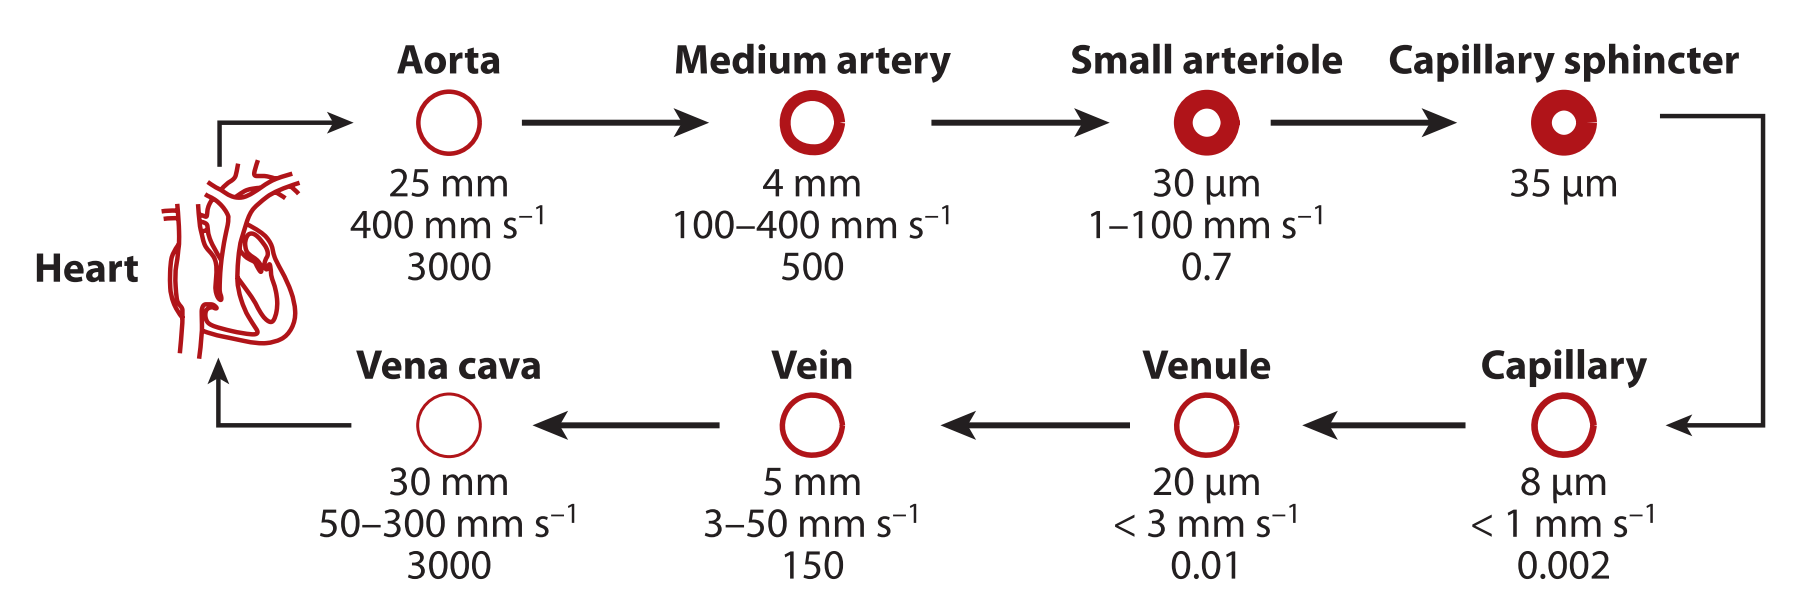
\includegraphics[width=1\textwidth]{Pictures/Bloodvessels.png}
%	\caption{Vessels of the cardiovascular systems and their properties: inner diameter, average blood-flow velocity, and Reynolds number from \cite{berger1996}}
%	\label{fig:veins}
%\end{figure}


\section{High Fields}

Mathematically this will be the easier case to solve. By assuming a very high applied field $\textbf{H}_\text{app}$ the ferromagnetic material will saturate, such that the magnetization becomes uniform:

\begin{equation}
\textbf{M}(\textbf{r}) = \textbf{M}_s \quad \forall \textbf{r}
\end{equation}

where $\textbf{M}_s$ points in the direction of the applied field and has magnitude $M_s$ which is the saturation magnetization of the material.

\begin{equation}
\textbf{M}_s = \frac{\textbf{H}_\text{app}}{|\textbf{H}_\text{app}|}M_s 
\end{equation}

\subsection{The Demagnetization Tensor}

We will now analyze how the demagnetization field looks like. We apply the high-fields case in its definition and we simplify:

\begin{equation}
\textbf{H}_d(\textbf{r}) = - \mathcal{N}(\textbf{r},\textbf{M}) = - \mathcal{N}(\textbf{r},\textbf{M}_s) = - \underbrace{\mathcal{N}(\textbf{r},I)}_{N(\textbf{r}):=}\textbf{M}_s
\end{equation}

Since we can take out the magnetization out of the integral operator we can define a tensor (by evaluating the integral over the identity matrix) that is only shape dependent. We will call this tensor, the demagnetization tensor. We can now write:


\begin{equation}
\textbf{H}_d(\textbf{r}) = -N(\textbf{r})\textbf{M}_s
\end{equation}

Which means that the total H-field is:

\begin{equation}
\textbf{H}(\textbf{r}) = -N(\textbf{r})\textbf{M}_s  + \textbf{H}_\text{app}
\end{equation}

\subsection{Analytical Calculation}

To calculate the demagnetization factor $N(\textbf{r})$ analytically, we only have to evaluate the integral operator defined above over the identity matrix:

\begin{equation}
N(\textbf{r}) := \mathcal{N}(\textbf{r},I) = \frac{1}{4\pi}\oint\limits_{\partial V}  \frac{(\textbf{r}'-\textbf{r})}{|\textbf{r}'-\textbf{r}|^3}\textbf{n}^T\;\mathrm{d}^2r'
\end{equation}


\subsection{Calculation over Simulation}

When performing a simulation with COMSOL, we set the material parameters as well as the shape of our bodies and subject them to the applied field. As an output, we get the H-Field as well as the magnetization in every point in the space. In the Appendix one can find the details to the simulation parameters used in COMSOL.\\

To calculate the demagnetization factor through the simulation, we use our integral equation and create three sets of linearly independent equations for three different linearly independent applied fields. Such that:

\begin{equation}
H(\textbf{r}) = -N(\textbf{r})M(\textbf{r}) + H_\text{app}
\end{equation}

where:

\begin{subequations}
\begin{equation}
H(\textbf{r}) := [\textbf{H}_1(\textbf{r}), \textbf{H}_2(\textbf{r}), \textbf{H}_3(\textbf{r})]
\end{equation}
\begin{equation}
M(\textbf{r}) := [\textbf{M}_1(\textbf{r}), \textbf{M}_2(\textbf{r}), \textbf{M}_3(\textbf{r})]
\end{equation}
\begin{equation}
H_\text{app} := [\textbf{H}_{\text{app},1}, \textbf{H}_{\text{app},2}, \textbf{H}_{\text{app},3}
\end{equation}
\end{subequations}

We solve to the demagnetization tensor and become:

\begin{equation}
N(\textbf{r}) = ( H_\text{app}-H(\textbf{r}) )M^{-1}
\end{equation}

If we're working with "high enough" applied fields, the magnetization will be approximately saturated. Since the applied fields are linearly independent the magnetization vectors will point in the direction of the correspondent applied fields, and thus will also be linearly independent, which makes the tensor $M$ nonsingular, such that its inverse always exists.\\

The problem with the method above, is that, depending on the shape, some directions at certain points in the body are more difficult to saturate. In other words they need much higher fields to achieve its saturation magnetization. However, COMSOL allows us to define a certain predefined, permanent magnetization for our helices. This is convenient to us, because we can avoid the step of adding an applied field by just forcing a certain constant magnetization over the whole body and using the relation between the magnetization and the demagnetization field it generates. Since a constant magnetization can only achieved through saturation, we can simulate a saturated body through setting a uniform magnetization. Similarly to the case above, we calculate the case for three linearly independant magnetizations (thus ensuring non-singularity on the demagnetization matrix) and calculate the demagnetization factor through the following relation:

\begin{equation}
H(\textbf{r}) = H_d(\textbf{r}) =  -N(\textbf{r})M
\end{equation}

The magnitude of the chosen magnetization will be canceled out by the proportional magnitude of the generated H-field. This is consistent with the fact of the demagnetization factor being just a form factor which doesn't depend on any field-related quantity. This is clear by reformulating the equation above:

\begin{equation}
N(\textbf{r}) = -H(\textbf{r})M^{-1}
\end{equation}

\subsubsection{Averaged Values}

Since we're dealing with the overall characteristics of a magnetic body, it makes sense to set the definitions of averaged values clearly. For example, the experimental results obtained through a VSM are of averaged nature. Also, most research papers that deal with demagnetization factors, assign one demagnetization matrix to a certain body (although, as we saw, there is a demagnetization factor for every point in it). It is convenient to use averaged values over the whole body and to be clear what are the characteristics of the its formal definition. In this section we will derive said definitions and its characteristics.\\

We define an averaging operator:

\begin{equation}
\langle \cdot \rangle := \frac{1}{V}\int\limits_V \cdot \;\text{d}^3r
\end{equation}

Where $V$ is the total volume of the body. We can now apply the definition to our integral equation:

\begin{equation}
\langle \textbf{H}(\textbf{r})\rangle = \langle-N(\textbf{r})\textbf{M}_s  + \textbf{H}_\text{app} \rangle
\end{equation}

which, using linearity of the average operator, leads to:

\begin{equation}
\langle \textbf{H}(\textbf{r})\rangle = -\langle N(\textbf{r}) \rangle\textbf{M}_s  + \textbf{H}_\text{app}
\end{equation}

We can use this to derive the calculations out of the simulations by applying the averaging operator on our simulation equations:

\begin{equation}
\langle N(\textbf{r}) \rangle = ( H_\text{app}-\langle H(\textbf{r})\rangle )M^{-1} 
\end{equation}

and

\begin{equation}
\langle N(\textbf{r}) \rangle = -\langle H(\textbf{r})\rangle M^{-1} 
\end{equation}

Which is a very interesting characteristic. It basically shows us that in order to calculate the average demagnetization tensor over the whole volume we simply calculate the average H-field instead of having to calculate the demagnetization tensor in every point and then averaging over the whole volume. \\

From now on, no explicit dependence of location is written next to a variable, matrix or field, we will assume it is an averaged value, e.g.:
\begin{equation}
N := \langle N(\textbf{r}) \rangle
\end{equation}


\subsection{Properties}

From the its definition, it is easy to see that the demagnetization tensor $N(\textbf{r})$ is symmetric and has therefore a set of orthonormal eigenvectors that diagonalize it it\footnote{If a matrix A is symmetric (i.e. $A^T = A$) its eigenvalues are orthogonal. Proof: We have two eigenvectors $\textbf{x}$ and $\textbf{y}$ with their respective eigenvalues $\lambda$ and $\mu$. We then have $A\textbf{x} = \lambda\textbf{x} \Rightarrow \textbf{y}^TA\textbf{x} = \textbf{y}^T \lambda\textbf{x} \Rightarrow (A^T\textbf{y})^T\textbf{x} = \textbf{y}^T \lambda\textbf{x}  \Rightarrow (A\textbf{y})^T\textbf{x} = \textbf{y}^T \lambda\textbf{x}  \Rightarrow \mu\textbf{y}^T\textbf{x} = \textbf{y}^T \lambda\textbf{x} \Rightarrow (\mu - \lambda)\textbf{y}^T\textbf{x} = 0 \Rightarrow \textbf{y}^T\textbf{x} = 0 $ }. \\

Another property proven in \cite{Schlomann1962} is that its trace always sums up to one:

\begin{equation}
\text{trace}(N(\textbf{r})) = 1 \quad \forall \textbf{r} \in V
\end{equation}

 Applying the average operator on both sides of the previous equation and exploiting its linearity as well as the linearity of the trace function we become:

\begin{equation}
\text{trace}(\langle N(\textbf{r})\rangle) = \text{trace}(N)= 1
\end{equation}

In other words, the trace of the averaged demagnetization tensor is also equals to one.\\

Later in the report, we will be able to proof mathematically that for soft-magnetic materials (not necessarily with high magnetic permeability) the demagnetization factor will directly tell us in what direction the body magnetizes the easiest, the so called `''easy axes'' of magnetization. In addition to this, when the body has high permeability, the eigenvalues of the demagnetization factor tell us directly which directions magnetize easier and which harder. Smaller eigenvalues means easier magnetization whereas higher values mean that the correspondent direction is harder to magnetize.

\subsection{Validation}
Our point of reference for every calculation, will always be the simulation with COMSOL. In order to be able to take the correctness of our simulations for granted we need to validate them for shapes where the integral operator can be solved and averaged in a closed form such that an algebraic formula can be used. This is the case for Ellipsoids and Rectangles.

\subsubsection{Rectangles}
The analytical value of the demagnetization matrix $N$ for a rectangular prism is calculated according to \cite{Aharoni1998}. \\

\begin{figure}[ht]
	\centering
  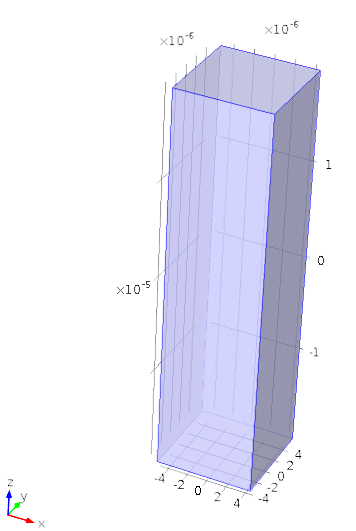
\includegraphics[width=0.4\textwidth]{Pictures/rectangle.png}
	\caption{Magnetic rectangle with displayed dimensions (in meter) for simulation in COMSOL}
	\label{fig:rectangle}
\end{figure}

After having used the formulate shown by \cite{Aharoni1998} and having calculated the (averaged) demagnetization tensors as well as the We compare the numerical calculation with COMSOL (see Figure \ref{fig:rectangle}) with the closed algebraically calculated value and become very little error (see Figure \ref{fig:N_rectangle}). We do the same with the Ellipsoids

\begin{figure}[ht]
	\centering
  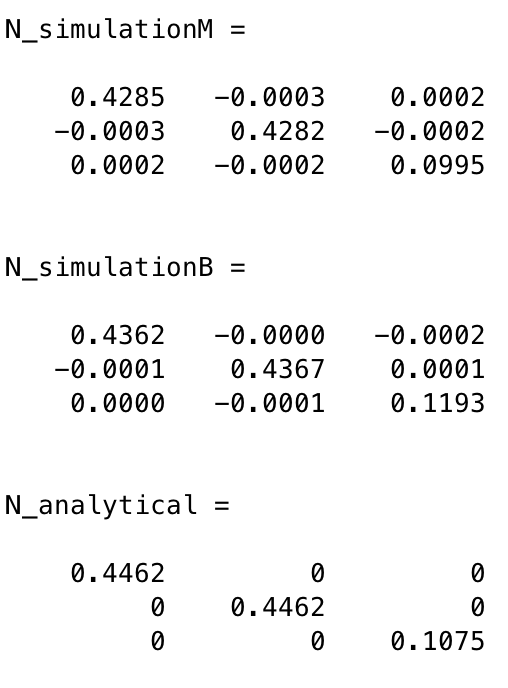
\includegraphics[width=0.4\textwidth]{Pictures/N_rectangle.png}
	\caption{Demagnetization matrices for a magnetic rectangle calculated trough the two explained methods in COMSOL and its analytical value}
	\label{fig:N_rectangle}
\end{figure}

\subsubsection{Ellipsoids}

Ellipsoids will not only help us validate our COMSOL environment, but it is a shape that shows interesting magnetic characteristics. First of all, it always magnetizes uniformly when put inside a uniform applied field. This means that every point in the body will have the same magnetization vector. This will be useful to analyze certain material characteristics when dealing with low applied fields. As a consequence of this, the demagnetization factor doesn't need to be averaged, since it's constant all over the body. \\

The second property is the fact that the demagnetization factor $N$ is a diagonal matrix if displayed in the coordinate system of the ellipsoid semi-axes. This means that the semi-axes of the ellipse are the eigenvalues of the matrix. In other words, an applied field in the direction of one of the ellipsoid axes will magnetize the ellipsoid in that specific direction.\\

\begin{figure}[ht]
	\centering
  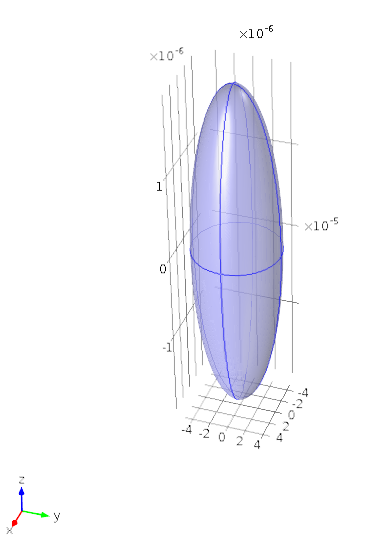
\includegraphics[width=0.4\textwidth]{Pictures/ellipsoid.png}
	\caption{Magnetic ellipsoid with displayed dimensions (in meter) for simulation in COMSOL}
	\label{fig:ellipsoid}
\end{figure}

In Figure \ref{fig:ellipsoid} we see the dimensions of the analyzed ellipsoid and in Figure \ref{fig:N_ellipsoid} the results of the calculations.\\

\begin{figure}[ht]
	\centering
  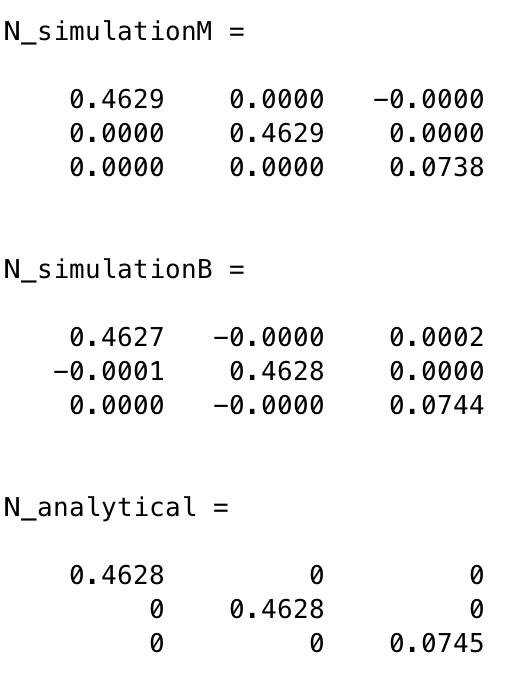
\includegraphics[width=0.4\textwidth]{Pictures/N_ellipsoid.png}
	\caption{Demagnetization matrices for a magnetic ellipsoid calculated trough the two explained methods in COMSOL and its analytical value}
	\label{fig:N_ellipsoid}
\end{figure}

Again, we were able to validate our COMSOL environment since the demagnetization matrices display little error.\\

The second property showed before regarding ellipsoids is used in the literature as a powerful tool to show the magnetization characteristics of other, more complicated magnetic bodies. Since every soft-magnetic body with high permeability will have a demagnetization factor $N$, it will also have easy axes of magnetization, which will be the eigenvalues of the matrix. Since the matrix can be diagonalized in the coordinate system of this easy axes, one can define a so-called ''equivalent ellipsoid'' which will not only have the same volume, but also the same easy axes, as well as the same ratio of the inverse-eigenvalues displayed by its semi-axes.\\

\begin{figure}[ht]
	\centering
  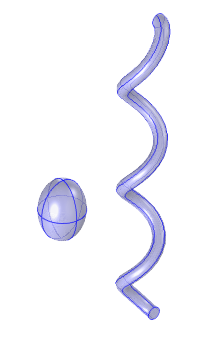
\includegraphics[width=0.25\textwidth]{Pictures/eqell.png}
	\caption{Equivalent ellipsoid of a helical soft-magnetic body with high permeability}
	\label{fig:eqell}
\end{figure}

Figure \ref{fig:eqell} shows the equivalent ellipsoid of a helical body with high permeability. From the direction and length of the body's semi-axes one can directly read that the most elongated  direction of the helix is the direction where it magnetizes the easiest. Whereas the two remaining easy-axes is where it would magnetize the hardest.


\subsection{Helical Bodies}

The real challenge of evaluating the demagnetization factor of our helices is an effective and efficient way of calculating this surface integral numerically. Matlab allows us to evaluate two-dimensional integrals in a straight forward way, but since our surface is curved we have to set up the integral in the appropriate coordinate system. \\


For the helical bodies, as we mentioned before, we assumed a soft-magnetic behavior with high permeability. We analyzed then the helices H1 to H10 being fully magnetic, thin coated and half coated and we compared the two methods exposed above, through numerical approximation of the surface integral as well as simulation.Since the axes of magnetization of the helices are almost aligned with the coordinate system, we will only present the diagonal values of the matrices.\\

\begin{figure}[ht]
	\centering
  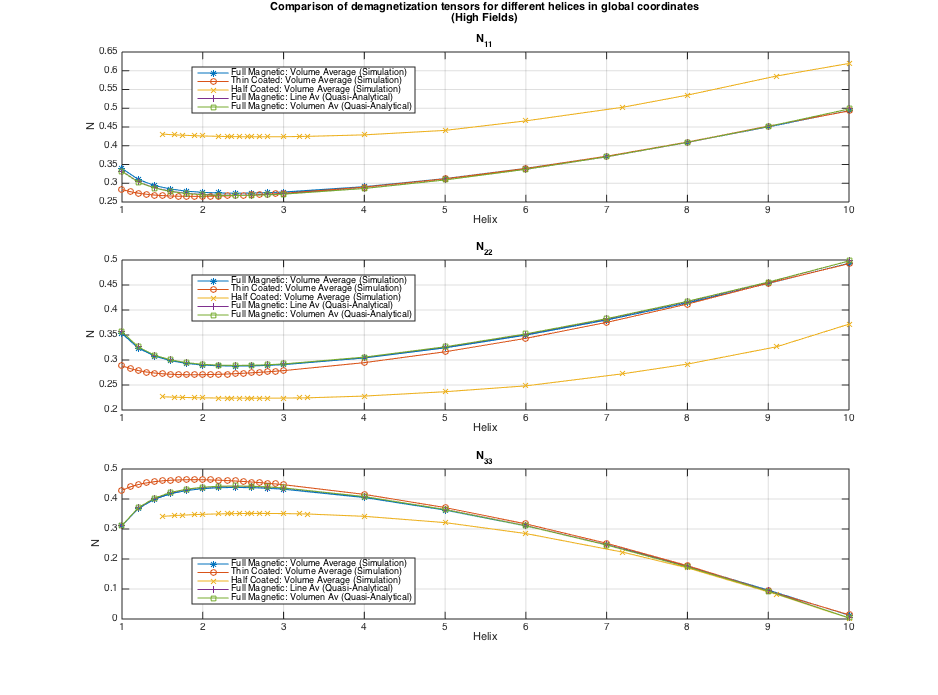
\includegraphics[width=1\textwidth]{Pictures/DemagFactors_Comparison_High.png}
	\caption{Diagonal values of demagnetization matrices of helical soft-magnetic helices with high permeability}
	\label{fig:DemagHigh}
\end{figure}

Figure \ref{fig:DemagHigh} shows said values for the simulations of full magnetic, thin coated and half coated helices against its quasi-analytical counterparts (numerical evaluation of the integral). For the case of half-coated helices, only a simulation was performed, since the mathematical definition of the magnetic volume for one sided thin coating was too complex. Since we are dealing with average values, in the case of the quasi-analytical calculation of the demagnetization factors, only a finite amount of points along the body where evaluated and then averaged. Additionally for the sake of comparison, a line average was done, where only points along the central line of the helix wire were calculated and averaged.\\

One can also see that for the case of the half-coated helices, different elongation indexes were used. The reason for this is the complexity of the meshing process in the simulation that often didn't allowed certain specific shapes. The method used to model the half-coated helices, was by subtracting two full helices which where shifted by a very small distance (200nm which is the coating thickness), thus leaving only a thin shell that resembles a half coated helix (See Figure \ref{fig:halfcoated}). \\

\begin{figure}[ht]
	\centering
  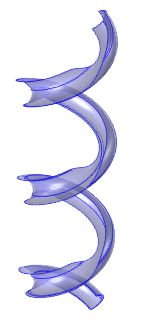
\includegraphics[width=0.2\textwidth]{Pictures/halfcoated.png}
	\caption{3D model of half coated elongated helix}
	\label{fig:halfcoated}
\end{figure}

The problem is that for coiled up elongations like H1, this method doesn't resemble the half-coating anymore and is therefore wrong (See Figure \ref{fig:halfcoatedcoiled}). That is the reason why shapes near H1 were not taken into consideration in the calculations.\\

\begin{figure}[ht]
	\centering
  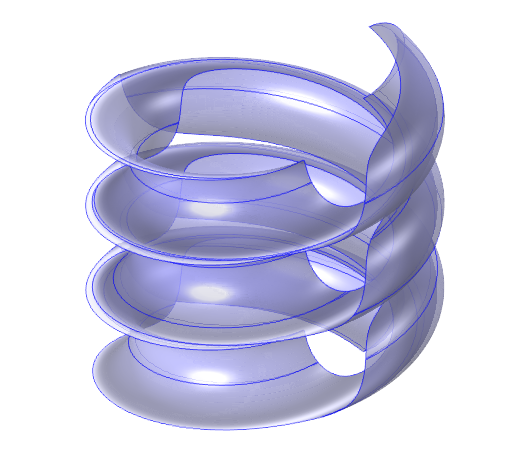
\includegraphics[width=0.2\textwidth]{Pictures/halfcoatedcoiled.png}
	\caption{3D model of half coated coiled-up helix}
	\label{fig:halfcoatedcoiled}
\end{figure}

For high permeabilities, one can calculate the misalignment angle of the helices towards its axes by analyzing the eigenvalues and eigenvectors of the demagnetization factor in the following fashion:

\begin{equation}
\theta = \arccos(\textbf{v}_\text{min})
\end{equation}

where $\textbf{v}_\text{min} $ is the normed eigenvector corresponding to the easy axes that is the easiest to magnetize, in other words, the one corresponding to the smallest eigenvalue of $N$. We plot then the angles and compare them to existing experimental data regarding the misalignment angles.\\

\begin{figure}[ht]
	\centering
  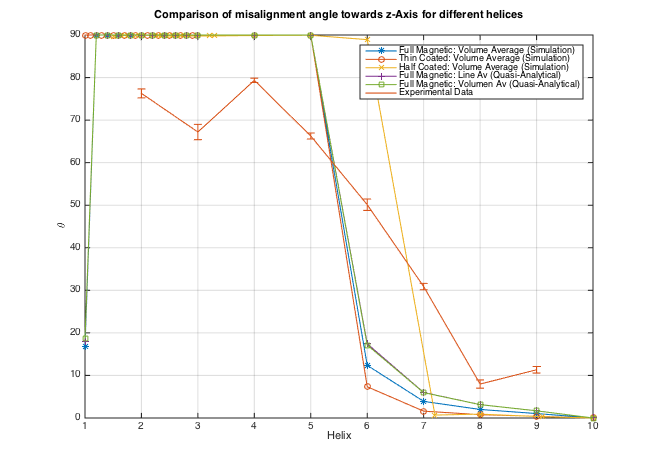
\includegraphics[width=1\textwidth]{Pictures/MisalignmentAngles_high.png}
	\caption{Misalignment angles of helical soft-magnetic helices with high permeability}
	\label{fig:MisalignmentAngles_high}
\end{figure}

FIgures \ref{fig:DemagHigh} and \ref{fig:MisalignmentAngles_high} help us see how accurate the quasi-analytical (numerical) calculation is compared to the simulations for full and thin helical bodies. We also see that the trend of the misalignment angle of the experimental results is captured by the simulations and quasi-analytical calculations.


\begin{figure}[ht]
	\centering
  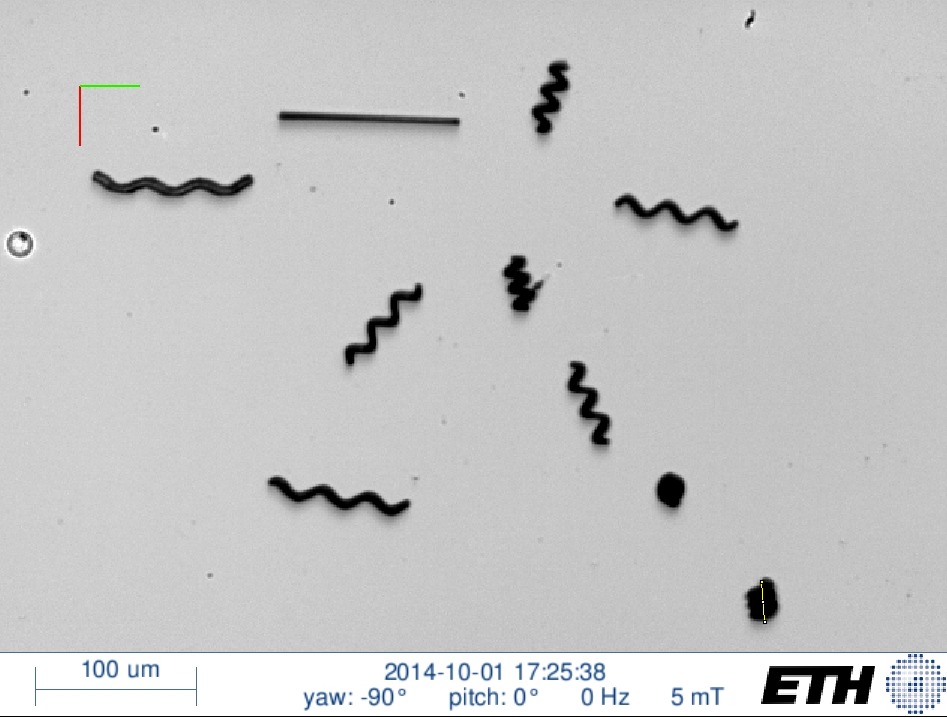
\includegraphics[width=0.8\textwidth]{Pictures/MisalignmentExperimental.png}
	\caption{Misalignment angles of helical soft-magnetic helices (experimental data)}
	\label{fig:MisalignmentExperimental}
\end{figure}


